\chapter{Specification}
\section{Purpose}
The prestudy of this thesis gives an insight into the fundamentals of messaging, especially
the purpose of message brokers for big data event streaming. We also compare
the most relevant broker implementations and provide detailed information about Apache
Kafka. The second part of this work is focusing on the implementation of a message
broker in the functional programming language \fnurl{Haskell}{https://www.haskell.org/}. 
The goal is to make use of the advantages of the functional paradigm regarding the resulting
throughput performance. By using the example of Apache Kafka, the main purpose
lies on building a server application which implements the main functionality of
Apache Kafka. 

\section{Components}

Basically, the architecture consists of two main components, namely the broker and
the client, whereas the client can act as producer, consumer or both. The broker
is a server which only reacts to requests that are sent from clients. Every
request contains an API key which the broker uses to determine which action it
has to do (e.g. persist produced message or consume message). For each valid
request the broker sends back a corresponding response to the client which
either includes the fetched data or an error code. The broker never communicates
with a client without a request.

\begin{figure}[H]
    \centering
     \begin{sequencediagram}
        %\newthread{broker}{Broker}
         \newinst[3]{client}{Client}
         \newinst[3]{broker}{Broker}
        \begin{messcall}
            {client}{(1) Send Request}{broker}{}
        \end{messcall}
        \begin{messcall}
            {broker}{(2) Do Action}{broker}{}
        \end{messcall}
        \begin{messcall}
            {broker}{(3) Send Response}{client}{} 
        \end{messcall}
     \end{sequencediagram}
     \caption{Basic communication between client (producer or consumer) and
     broker}
\end{figure}

Both, the client and broker component need to use the same underlying protocol
for communication. Because Apache Kafka is used as the benchmark for this project
and compatibility to existing Kafka clients is to be provided, the Kafka
Protocol version 0.8.x has been chosen to be implemented. Therefore, a third
component which fully implements this protocol is introduced additionally. It
exposes the appropriate functions and types as a library. This component fully
separates the clients from the broker. 

To support interoperability, the implementation of a client should be simplified
as much as possible. Therefore we provide a client library which provides functionalities to
easily implement a Haskell client for a Kafka-based broker. The goal of this, is to be able to
set up a client without knowing too many details about the Apache Kafka protocol
itself.

\begin{figure}[H]
    \centering
    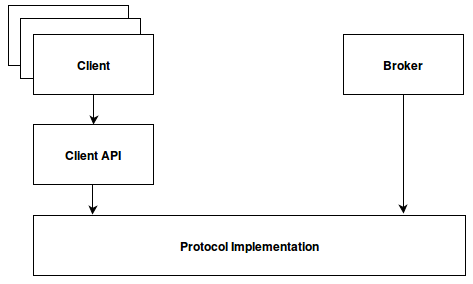
\includegraphics[width=0.55\textwidth]{images/architecture-components.png}
    \caption{Separation of code}
    \label{fig:architecture-components.png}
\end{figure}

\section{Workflow}

The main purpose of this broker implementation can be split in two cases. Case
one covers producing a message and persisting in the broker's log. Case two
allows to consume persisted messages on request. As for clients, depending on
which API is to be used, the client can act either as producer or consumer.

\subsection{Produce Messages}

In the case of a producer client, the following workflow highlights the
fundamental steps being passed from sending a request by the client to
persisting the message on the broker.

\begin{figure}[H]
    \centering
    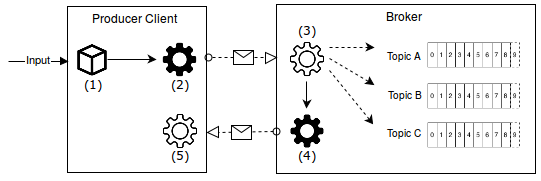
\includegraphics[width=0.8\textwidth]{images/concept_producer.png}
    \caption{Case one: Producer Workflow}
    \label{fig:conept-producer}
\end{figure}

\begin{description}
    \item [(1)] 
        {Packing Produce Request: Transforming input data into protocol-conforming data structure.}
    \item [(2)] 
        {Serializing and sending Produce Request: Encoding data structure to an
            binary  string and transmit over a tcp socket to the broker.}
    \item [(3)] 
        {Parsing and Handling Produce Request: Broker receives the binary string
            and parses it back to the appropriate data structure. The request
            handler of the  broker checks the API Key of the request. If it is a
            produce request, the containing message will be written to the
            appropriate topic log.}
    \item [(4)] 
        {Send Produce Response: A response is packed, serialized and transmitted
            back to the client. The response contains an error code which has
            the value 0 if everything worked well, otherwise another value for a
            specific problem. }
    \item [(5)] 
        {Parse Produce Response: Producer client receives a binary string and
            parses it to a valid response data structure }
\end{description}

\subsection{Consume Messages}

In the case where the client acts as a consumer, the workflow is not different from the one for
producing a message. Instead of the translation from request message to the log, persisted messages
are read from the log and are delivered from the broker to the client.

\begin{figure}[H]
    \centering
   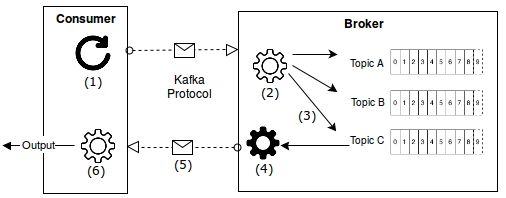
\includegraphics[width=0.7\textwidth]{images/concept_consumer.png}
    \caption{Case two: Consumer Workflow}
    \label{fig:concept-consumer}
\end{figure}

\begin{description}
    \item [(1)] 
        {Continuously send fetch request: Consumer client sends fetch
        requests in configurable interval as a binary string to the broker. } 
    \item [(2)] 
        {Parsing and handling fetch request: Broker receives the binary string
            and parses it back to the appropriate data structure. The request
            handler of the broker checks the API Key of the request. If it is a
            fetch request, the broker reads messages of the requested topic and
            packs them to a fetch response. The message will be written to the
            appropriate topic log.}
    \item [(3)] 
        {Send fetch response: The fetch request which contains the requested
        messages is sent back to the consumer client.}
    \item [(4)] 
        {Parse Response: Consumer client receives a binary string and parses it
        to a valid response data structure. }
\end{description}

